%======================================================================
\subsection{BW-ROU-05 --- Built, 30 Oct: pins and ports, routes that leave them straight, terminals in the BOM, fittings}\label{sec:rou05-built}
%======================================================================

Step~1 of the routing plan (\S\ref{sec:rou-next-plan}), with your answers C1--C3, F1 and F2 and the 30 Oct answers
on terminals and the BOM, was built in seven commits: \code{b54364a4} (the pin and port frames),
\code{ff18404f} (fittings), \code{3993e55d} (routes on frames, from-to, terminals), \code{8fa2750e} (terminals by
manufacturer and MPN), \code{4ba71a2c} (ROU-04: Length added to existing BOMs), \code{36d11732} (the Routing tab
commands) and \code{16279019} (a fix found from a render). The maths stays FreeCAD-free:
\file{addons/BruceWorx/bruceworx/routing.py} (leads, clamped splines, straight lengths, gauge ranges, the terminal
list) and the new \file{bruceworx/fittings.py} (size tables and fitting layouts). The FreeCAD side is the new
\file{bruceworx\_routing\_ports.py} (the frame schema, shared with the connector library of
\S\ref{sec:connlib-built}) and \file{bruceworx\_fittings.py}, plus changes to \file{bruceworx\_routing.py},
\file{bruceworx\_routing\_gui.py} and the vault BOM walker \file{bruceworx\_bom.py}; the Assembly BOM change is in
\file{src/Mod/Assembly/App/BomObject.cpp}, marked \code{[BW]}.

\begin{figure}[!htbp]
\centering
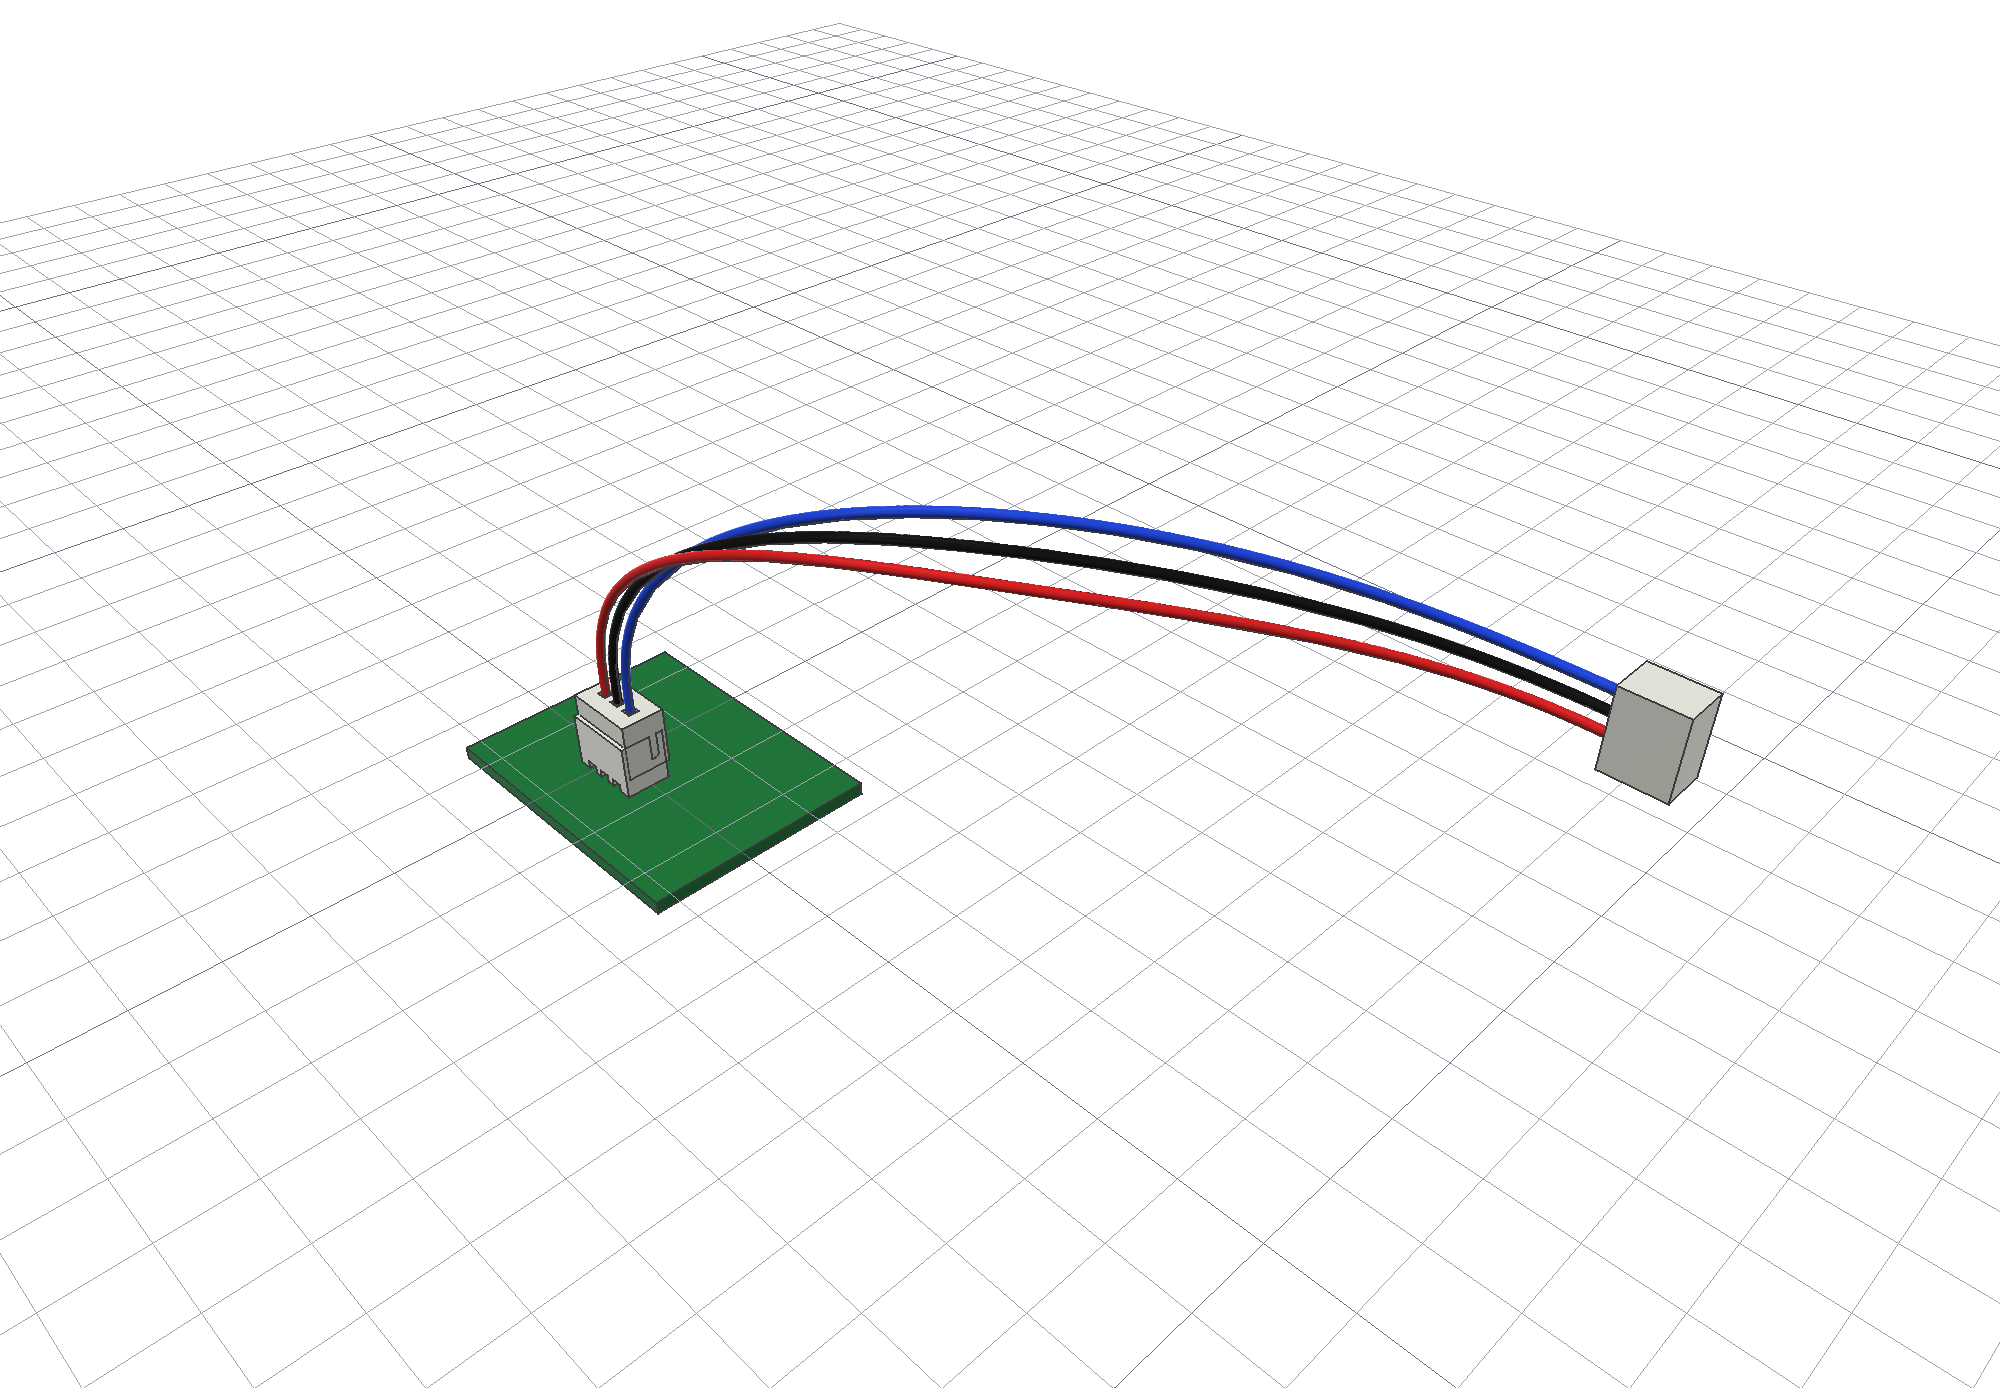
\includegraphics[width=0.49\linewidth]{fig/rou05_harness.png}\hfill
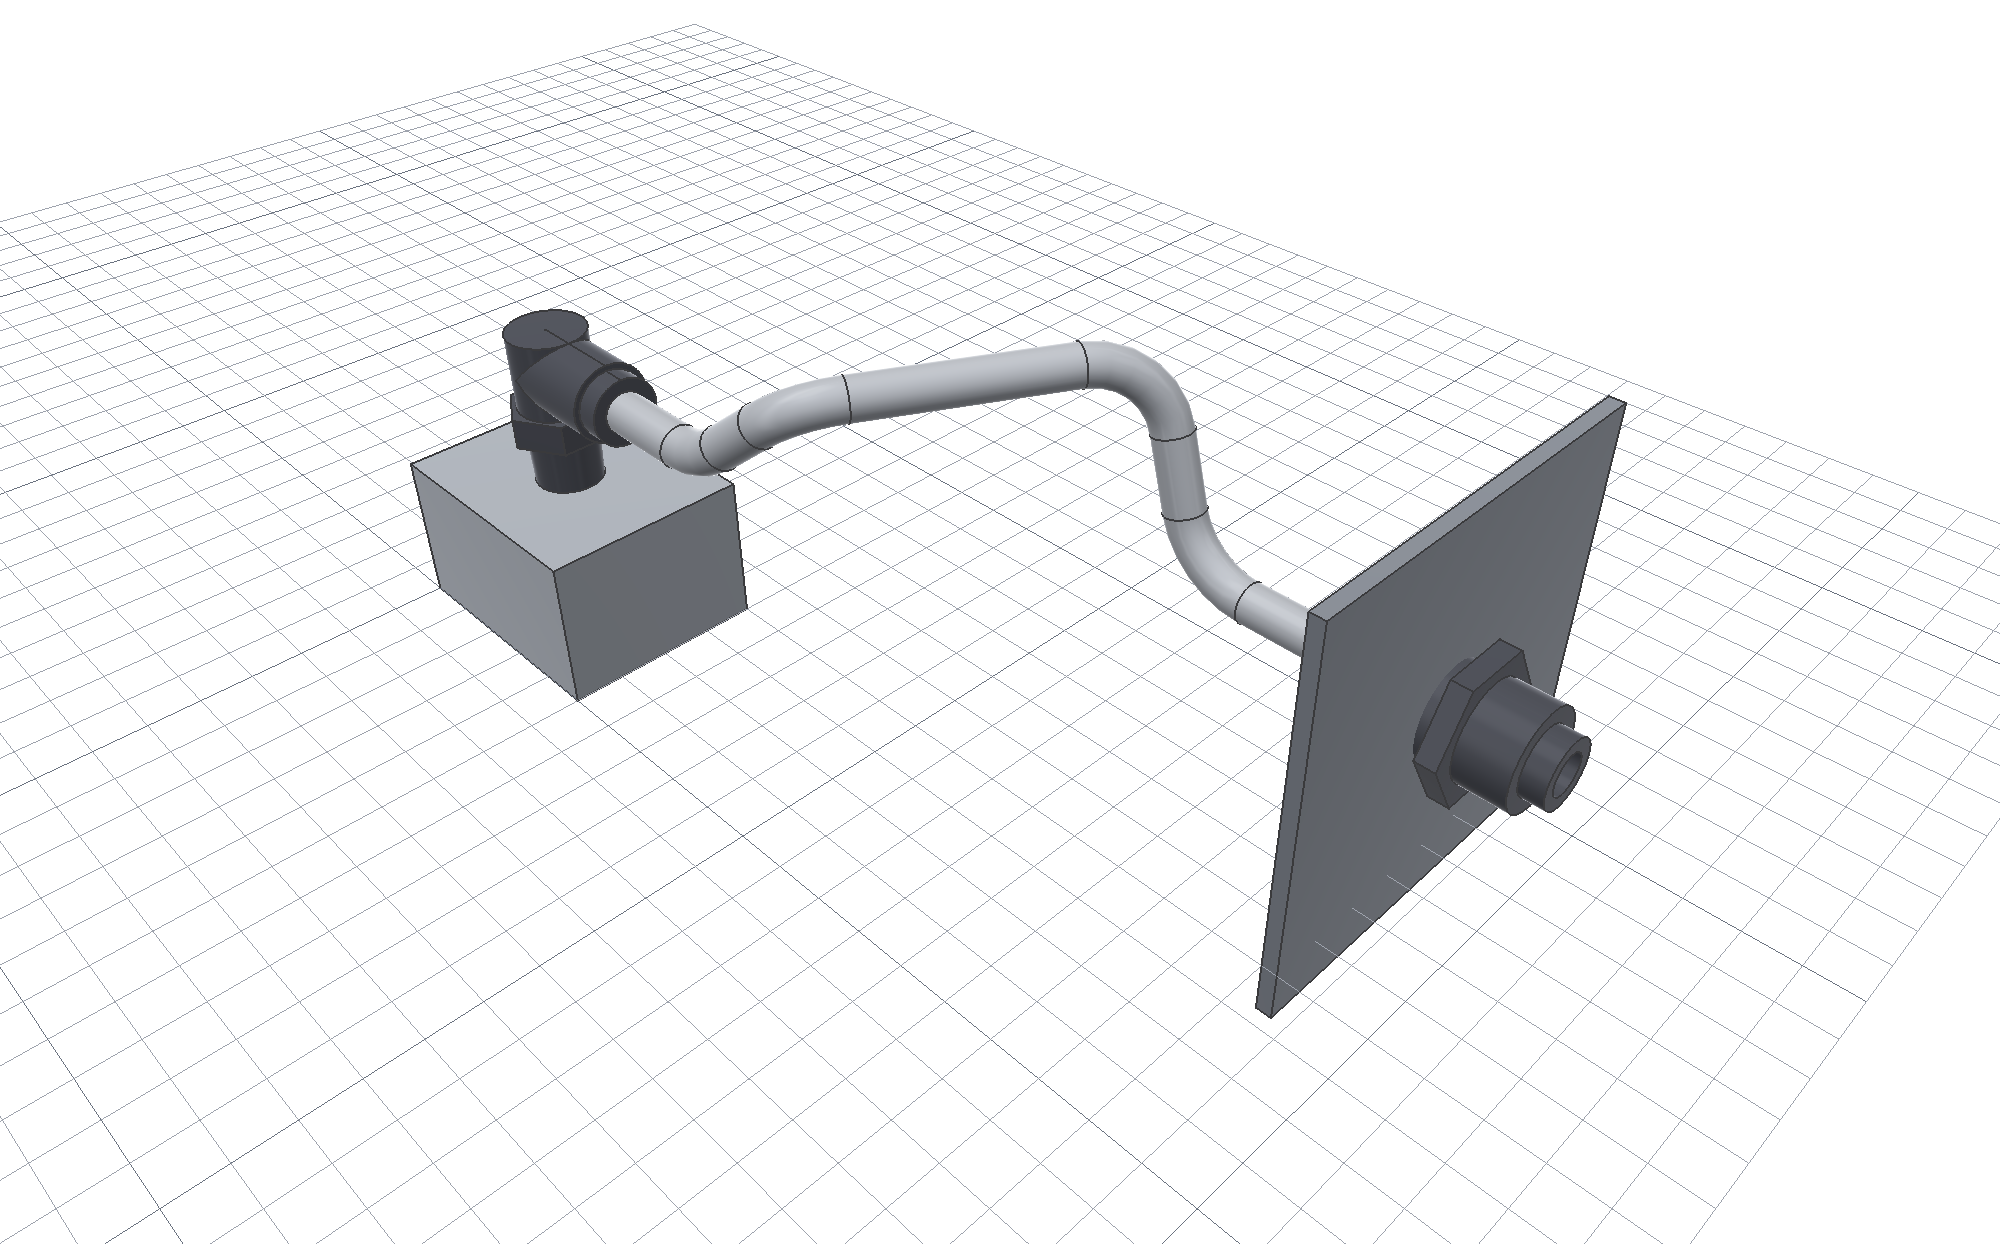
\includegraphics[width=0.49\linewidth]{fig/rou05_tube.png}
\caption{Left: three 22\,AWG wires from a JST XHP-3 housing (J1, mated on its B3B-XH-A header P1) to a second XHP-3
(J2), both real parts of the connector library, linked into an assembly. Each wire leaves its pin straight along
$+Z$ for $2\times$OD $=2.28$\,mm before the spline bends, and fills its from-to by itself: \code{J1, 1, P1 $\to$ J2,
1} (the mate column names P1); the terminal list reads \code{Terminal, SXH-001T-P0.6, 6}. Right: an 8\,mm tube from a
push-to-connect elbow screwed into a manifold (placed on the top face by the Fitting command) to a bulkhead union in
a panel, in Polyline mode at CLR 16: both ends leave straight for $2\times$OD $=16$\,mm, the cut length is
$169.5 + 2\times19 = 207.5$\,mm (19\,mm of tube inside each fitting). Off-screen renders of the real objects.}
\label{fig:rou05-built}
\end{figure}

\paragraph{What you can do now.}
\begin{itemize}[nosep]
  \item \textbf{Pin and port frames.} A connector or fitting is an ordinary \code{App::Part} with one
        \code{App::LocalCoordinateSystem} per pin or port, recognised by its \code{BWFrame} property. The origin is
        where the wire or tube enters (a contact cavity's rear face, a solder-cup mouth, a socket mouth, a barb tip),
        $+Z$ points out of the part the way the wire leaves. The schema (table below) is what the connector library
        generates; \textbf{Pin / Port} (Routing tab, new \emph{Parts} group) puts one on a hand-made part: pick a
        face (its centre, $+Z$ along its normal), a hole edge (its centre and axis, out of the solid) or a vertex;
        select an LCS to edit it (figure~\ref{fig:rou05-panels}).
  \item \textbf{Routes attach and leave straight} (F2). A Route Path whose first or last pick is on a pin or port
        (a click on the LCS or one of its axes, through an \code{App::Link} in an assembly too) attaches to it with
        the existing mechanism and \emph{leaves along $+Z$} for the straight length before the first bend: the
        frame's own \code{StraightLength}, else the defaults in \textbf{Bend Rules}: wires $2\times$OD past the
        terminal, hoses $2\times$OD, tubes $2\times$OD or the bender's clamp length if larger (the OD of the
        largest item on the path; with no item yet, the pin's thickest wire or the port's tube). The panel says
        ``Starts on Pin 1 of J1, straight 2.3\,mm''; \emph{Leave pins and ports straight} turns it off per path.
        A new path whose picks are inside an assembly goes into that assembly, so its wires are BOM lines there.
  \item \textbf{From-to by itself.} A wire on such a path fills \code{From}, \code{From pin}, \code{To},
        \code{To pin} from the connector instance's label (J1, the link, not the part file) and the pin name, and
        \code{Signal} from the pin's default signal. Whatever you type over them stays; the rest keep following.
        A wire outside the pin's gauge range gets a \code{Warnings} line and a ``gauge'' badge in the Browser.
        The from-to CSV has \emph{From mate} and \emph{To mate}: the connector each end's connector is mated
        with, when both halves are in the document.
  \item \textbf{Terminals in the BOM} (C3 and your 30 Oct answer). One terminal and one seal per wire end on a pin,
        and a connector's \code{Accessories} (a Deutsch wedgelock) once per instance. Ordered by
        \emph{manufacturer and MPN}; the Standard Library number is how the vault finds them. The vault BOM walker
        keys each line by the STD item, then the MPN, and names it ``Terminal: JST SXH-001T-P0.6 (STD-\dots)'';
        \textbf{Terminal list} (Reports) writes a CSV with \emph{Kind, Manufacturer, MPN, Standard Library item,
        Qty} in columns of their own.
  \item \textbf{Fittings} (F1, all four families), parametric from size tables, each an \code{App::Part} with a
        \code{FittingBody} and its port frames (figure~\ref{fig:rou05-fittings}). \textbf{Fitting} (Parts group)
        has a family, style, size and thread picker, live, placed on the selection: its thread (else port 1)
        goes on the picked face, hole edge or port, facing into it. Changing style or size rebuilds the shape and
        moves, adds or removes the ports; the description (``Push-to-connect male elbow, 6\,mm tube x 1/8 BSPP''),
        a generic type code (\code{PTC-ELBOW-6MM-1/8BSPP}, not a vendor's) and the part-property schema
        (\code{PartNumber}, \code{Vendor}, \code{VendorPartNumber}, \dots) make it P/N-ready. A port's
        \code{Engagement} (tube inside the fitting, hose over the barb) is added to a pipe's cut length and its
        first and last feed in the bend table, and to a hose's length.
  \item \textbf{Assembly BOM Length on old BOMs} (your 30 Oct answer to ROU open question~5): a BOM saved before
        the Length column gets it once when its file is opened; one whose columns you changed since keeps them.
\end{itemize}

\begin{center}
\small
\begin{tabularx}{\linewidth}{@{}llX@{}}
\toprule
Frame & Property & Meaning \\
\midrule
Pin & \code{PinName} & as on the datasheet or footprint pad (1, A3, VBAT) \\
    & \code{GaugeMin}, \code{GaugeMax} & thinnest and thickest wire, AWG (28 and 22); 0 = not stated \\
    & \code{TerminalPN}, \code{TerminalMfr}, \code{TerminalItem} & terminal MPN (ordered), manufacturer, STD item \\
    & \code{SealPN}, \code{SealMfr}, \code{SealItem} & the same for the wire seal \\
    & \code{DefaultSignal}, \code{StraightLength} & signal a wire gets; straight before the bend (0 = rule) \\
Port & \code{PortName}, \code{PortType} & 1, 2, IN; push-to-connect, barb, compression, NPT, BSPP, metric, UNF \\
    & \code{PortSize}, \code{TubeOD} & 6\,mm, 1/8 NPT; the tube it takes (barb: hose ID) \\
    & \code{StraightLength}, \code{Engagement} & straight before the bend; tube inside the fitting \\
Part & \code{ConnectorFamily}, \code{ConnectorRole} & JST-XH, push-to-connect; wire housing, header, fitting \\
    & \code{MatingPN}, \code{FrameAt} & mating half's P/N(s), \code{;}-separated; where header pins sit \\
    & \code{Accessories} & once per instance: \code{MPN|Manufacturer|STD item|qty|kind} \\
\bottomrule
\end{tabularx}
\end{center}

\begin{figure}[!htbp]
\centering
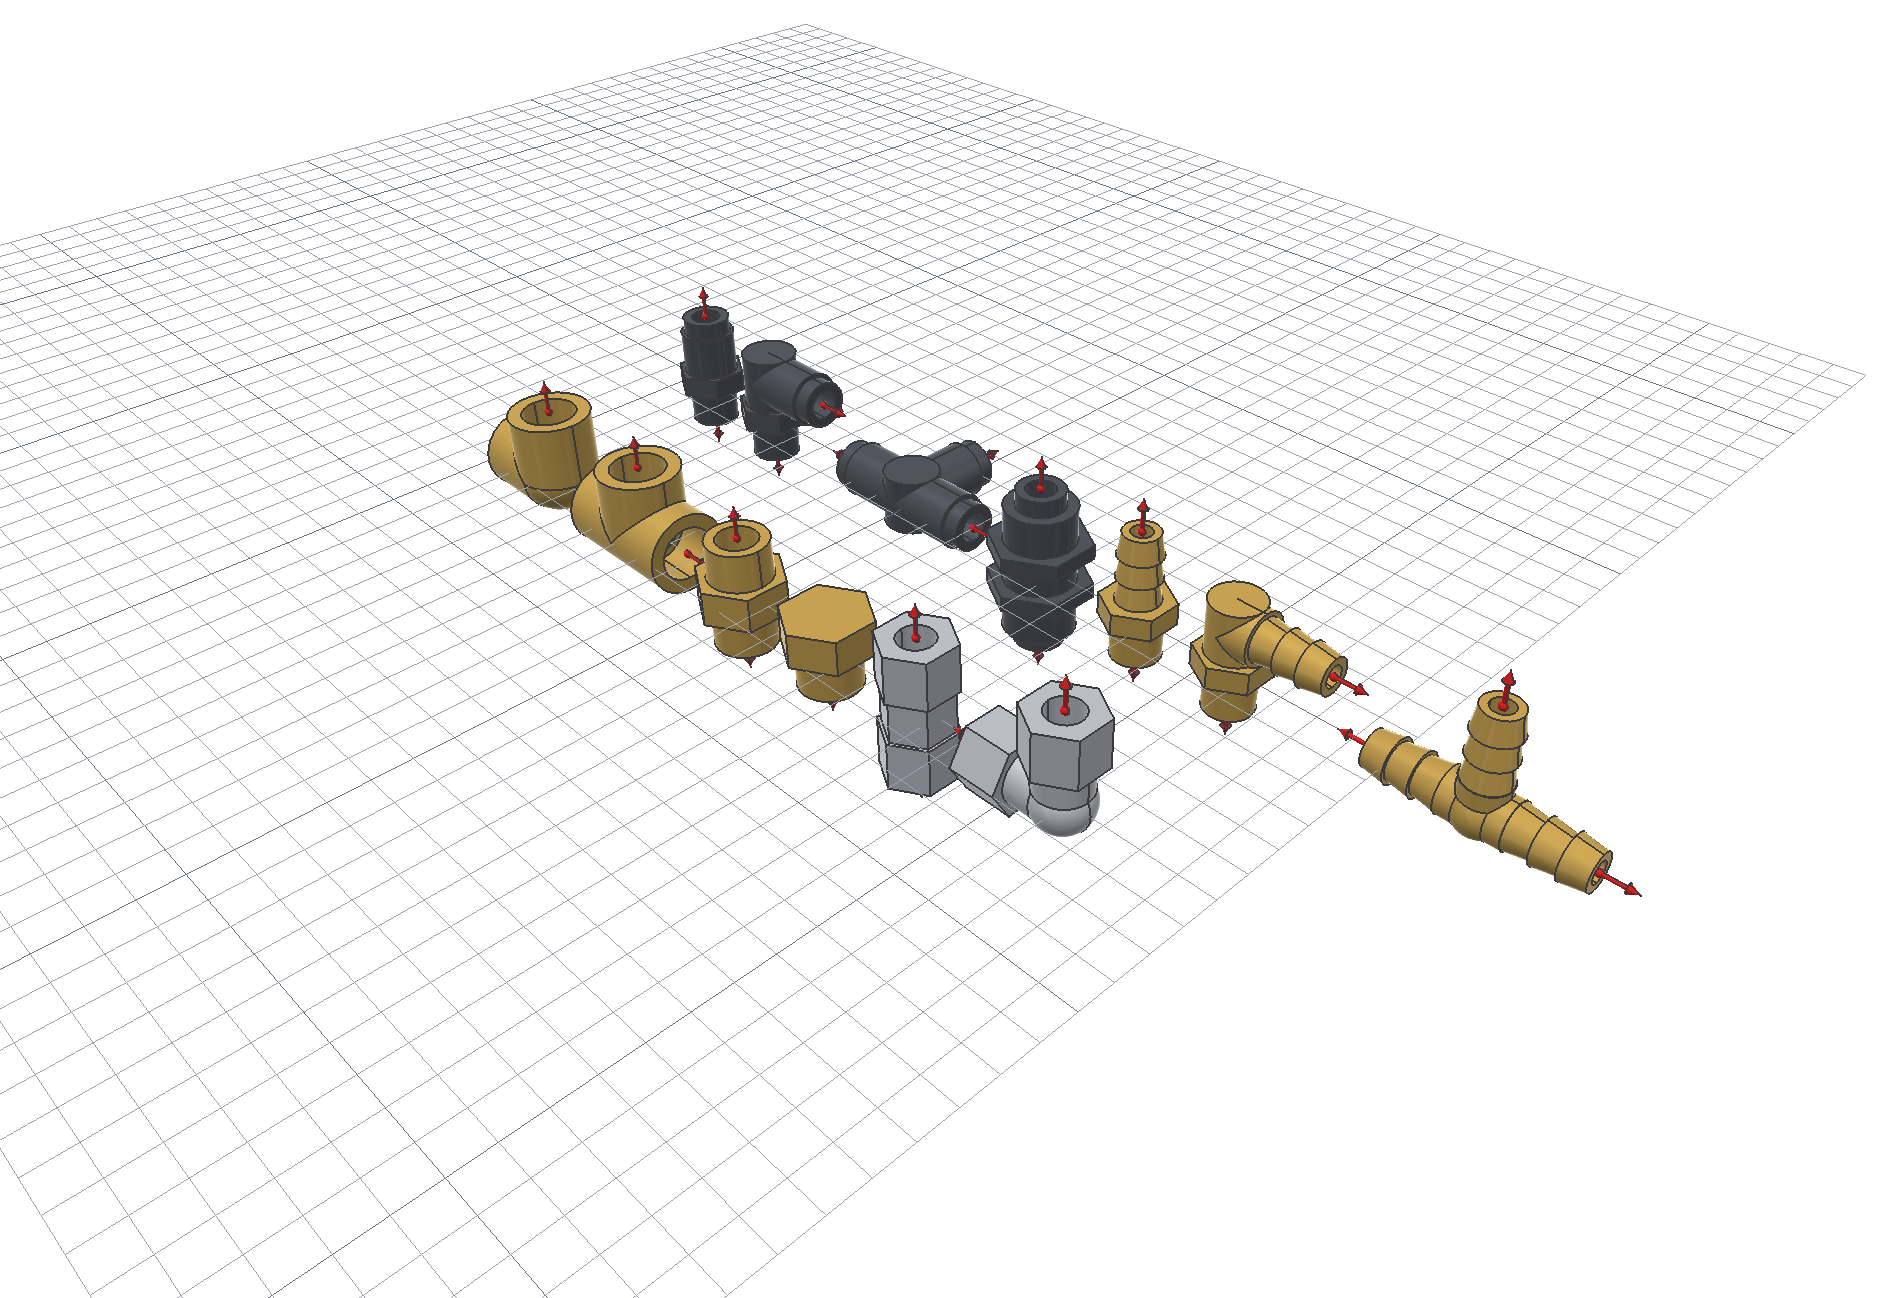
\includegraphics[width=0.92\linewidth]{fig/rou05_fittings.png}
\caption{One of each fitting with its port frames as red arrows ($+Z$, the way the tube leaves): push-to-connect
male connector, male elbow, union tee and bulkhead union (8\,mm, 1/4 NPT); hose barbs straight and elbow on 1/4 NPT
and a barb tee (3/8\,in); NPT female elbow, tee, hex nipple and plug (3/8); compression union and union elbow
(3/8\,in). Off-screen render of the real parametric parts.}
\label{fig:rou05-fittings}
\end{figure}

\begin{figure}[!htbp]
\centering
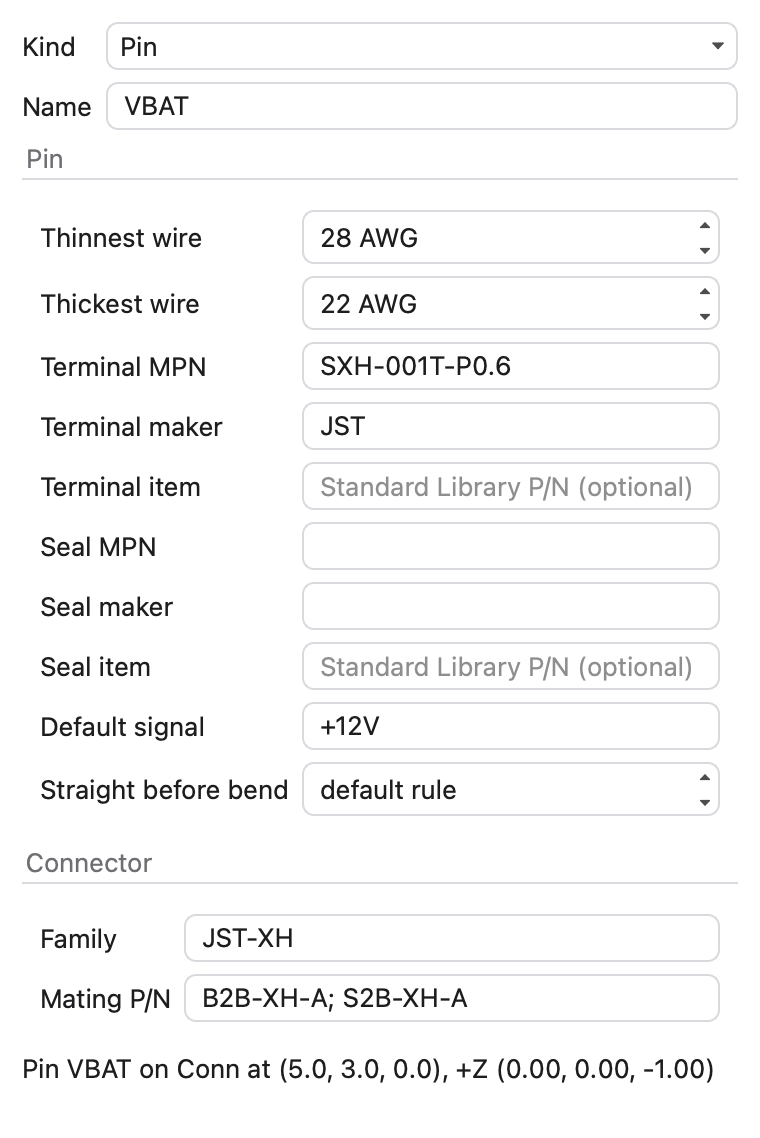
\includegraphics[width=0.36\linewidth]{fig/rou05_framepanel.png}\hfill
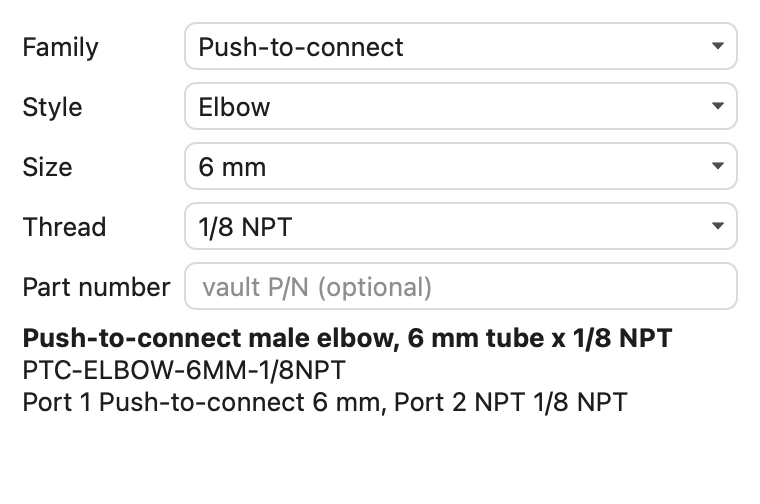
\includegraphics[width=0.36\linewidth]{fig/rou05_fittingpanel.png}\hfill
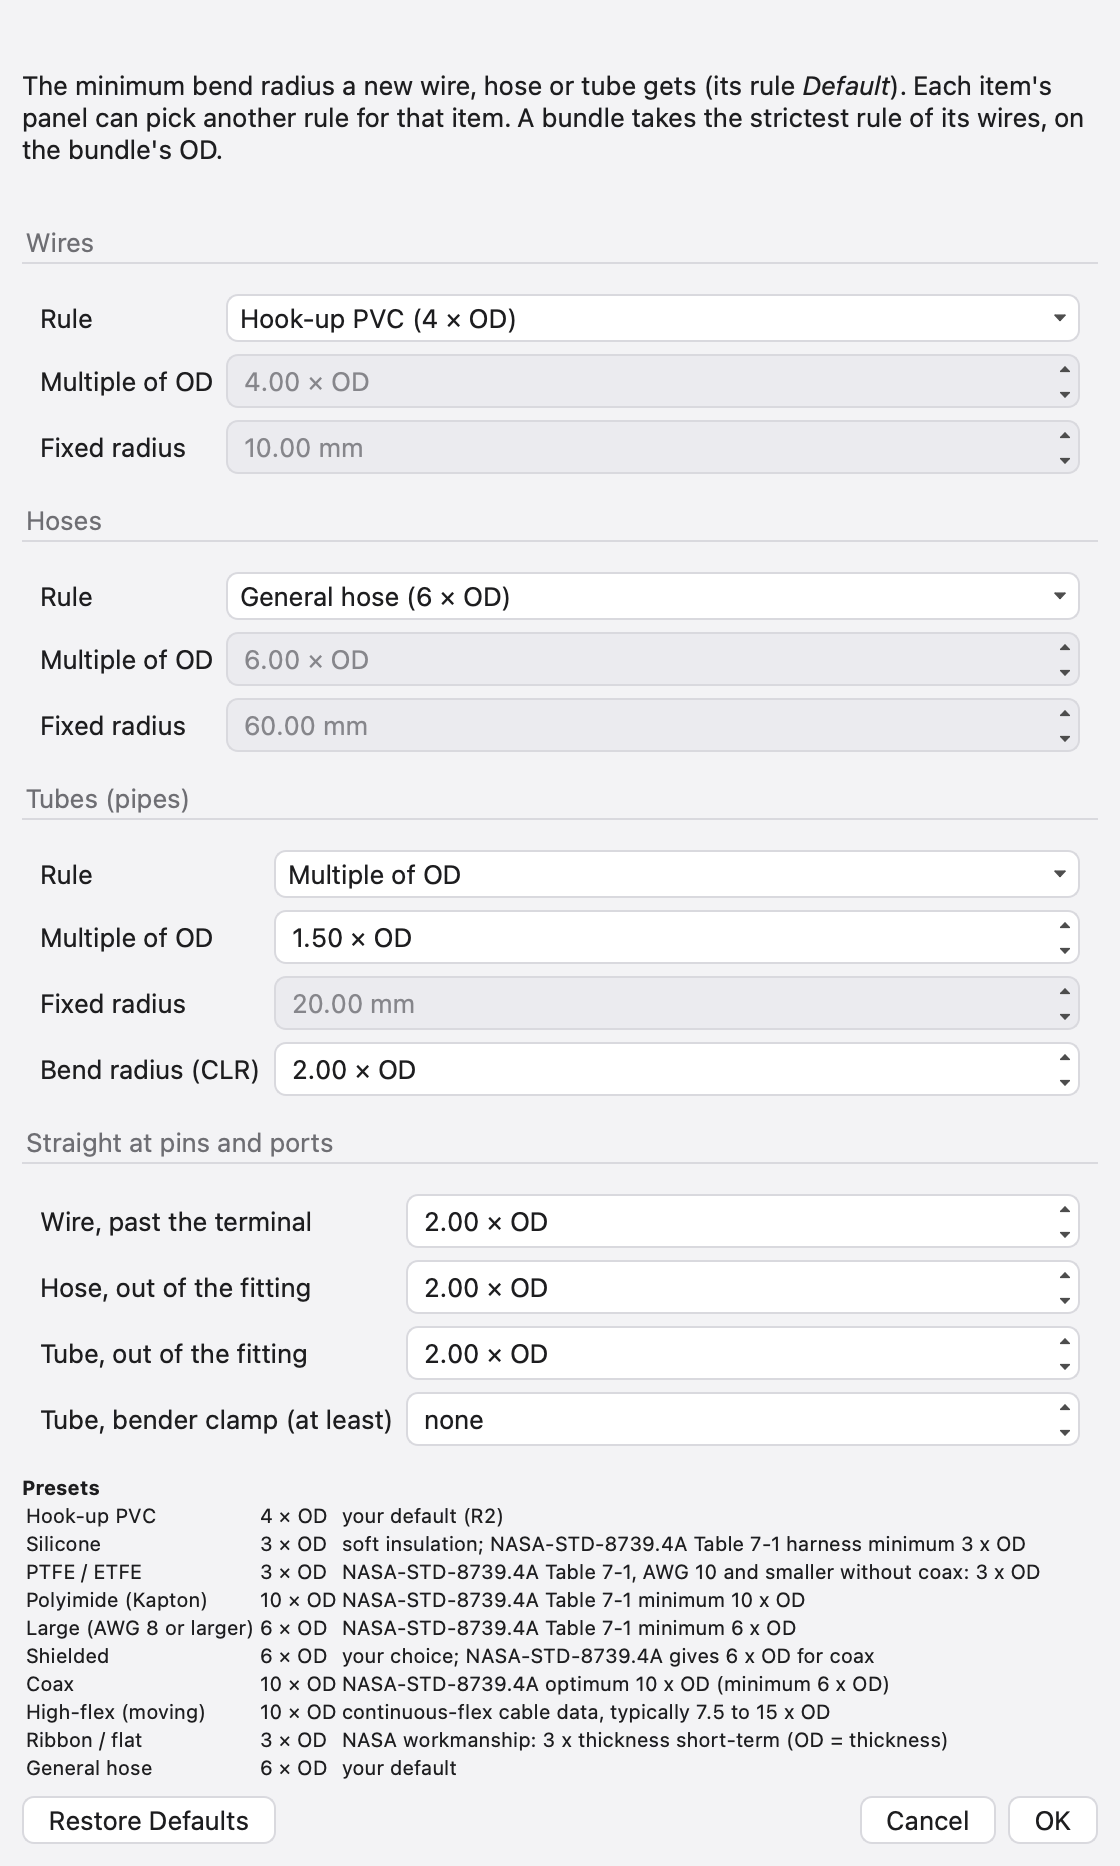
\includegraphics[width=0.26\linewidth]{fig/rou05_bendrules.png}
\caption{Left: the Pin / Port panel on a hand-made housing (pin VBAT, 28--22\,AWG, terminal MPN and maker, the
connector's family and two mating P/Ns). Middle: the Fitting panel placing a push-to-connect elbow on a picked face.
Right: Bend Rules with the new \emph{Straight at pins and ports} group. Off-screen grabs of the real widgets.}
\label{fig:rou05-panels}
\end{figure}

\paragraph{The straight at a frame.} For a lead of length $L$ out of a frame at $\mathbf O$ along $\mathbf d$ ($+Z$):
\begin{itemize}[nosep]
  \item \emph{Spline mode:} a line $\mathbf O\to\mathbf Q=\mathbf O+L\mathbf d$, then the spline from $\mathbf Q$
        through the other points with its first derivative \emph{clamped} to $\mathbf d$:
        $2h_0M_0+h_0M_1=6\bigl((y_1-y_0)/h_0-d\bigr)$ replaces the not-a-knot row (its mirror at the end, arriving
        along $-Z$). The chord-length spline leaves $\mathbf Q$ at unit speed and the line runs at unit speed, so the
        joins are $C^1$ and the whole route is \emph{one} clamped cubic B-spline (each line a Bézier at its thirds,
        joined at a knot of multiplicity 3). OCC failed to sweep a line--spline--line wire
        (\code{BRepFill\_Sweep::BuildEdge}); one edge sweeps. The bend check measures the curvature of that curve,
        so a pin facing away from the route is flagged (the spline has to turn back right after the straight).
  \item \emph{Polyline mode:} the lead end becomes a corner at $\mathbf Q=\mathbf O+(L+t)\mathbf d$ with
        $t=R\tan(\theta/2)$, so the arc starts exactly $L$ out. $\theta$ depends on $\mathbf Q$ (and with two points,
        on the other lead): a fixed-point iteration, a handful of steps. A next point behind the frame
        ($\theta>90^\circ$) caps $t$ at $R$, and the corner that then does not fit is reported, not chased outwards.
        A first or last straight shorter than its lead is a problem in \code{Problems}.
\end{itemize}

\paragraph{Fitting dimensions and their sources.}
\begin{center}
\small
\begin{tabularx}{\linewidth}{@{}lX@{}}
\toprule
Data & Source \\
\midrule
NPT 1/8--1/2 & ASME B1.20.1: pipe OD at the thread $D$ = 0.405, 0.540, 0.675, 0.840\,in; 27, 18, 18, 14 TPI;
               effective thread $L_2$ = 0.2639, 0.4018, 0.4078, 0.5337\,in; taper 1 in 16 on the diameter (drawn as
               a cone). Tap drills 11/32, 7/16, 37/64, 23/32\,in from the usual tap-drill charts. \\
BSPP 1/8--1/2 & ISO 228-1: major diameter 9.728, 13.157, 16.662, 20.955\,mm; 28, 19, 19, 14 TPI. Male thread
               lengths (8, 11, 12, 15\,mm) are typical catalogue values, approximate. M5\,$\times$\,0.8: ISO metric. \\
Push-to-connect & 4--12\,mm and 5/32--3/8\,in: body diameters (10.4, 12.8, 15.2, 18.5, 20.9\,mm for 4--12) and
               lengths in the style of the SMC KQ2 / Festo QS catalogue tables, from memory and rounded; insertion
               depth approximated as OD\,+\,11\,mm. \\
Compression & Nut hexes 7/16, 9/16, 11/16, 7/8\,in for 1/8--1/2\,in tube as in Swagelok-style catalogues; metric nut
               hexes 12--22\,mm, body hexes and insertion depths ($0.6\,$OD$+4$) approximate. \\
Barbs & No standard governs barbs: crest about 20\,\% over the hose ID, bore 60\,\%, length $\max(8, 1.8\,\mathrm{ID}+2)$. \\
Hexes, elbow centres & typical catalogue proportions, approximate. \\
\bottomrule
\end{tabularx}
\end{center}
Only the NPT and BSPP numbers are from the standards themselves; everything else is for layout and routing (where
the tube enters, how much straight it needs, what the BOM says), not for manufacture. Check the vendor drawing before
release, as the module docstring says.

\paragraph{Decided while building.}
\begin{itemize}[nosep]
  \item \textbf{A frame is recognised by a property, not a name.} Pin names like ``+12V'' are not valid object
        names (FreeCAD makes \code{Pin\_12V}); \code{BWFrame} plus \code{PinName} keep the datasheet name.
  \item \textbf{The connector is the instance.} \code{frame\_at} walks the pick's path and takes the nearest
        \code{App::Link} above the frame (J1 in the assembly), else the frame's own part; the from-to and the mate
        use its label. Two identical housings on two identical headers pair nearest first, each in one pair only.
  \item \textbf{Picks are re-rooted} below the path's own containers: a 3D pick arrives as (assembly,
        ``J1.Pin1.''), and a path inside that assembly linking to the assembly would be a dependency cycle. The
        point is the same; only the anchor moves down.
  \item \textbf{The straight follows the item.} The path reads the OD of the items on it (a wire changing gauge or
        insulation touches its path), so one pin gives $2\times1.14$ for a 22\,AWG wire and $2\times1.6$ for a
        thicker one; a frame's own \code{StraightLength} always wins.
  \item \textbf{Terminals are a property list, not objects.} \code{BomExtras} on the wire
        (\code{key|qty|kind|manufacturer|MPN}) carries what the BOM needs without terminal objects in the tree; the
        walker counts them under whatever multiplies the wire. The connector library agreed the v1.2 fields
        (\code{TerminalMfr}, \code{TerminalItem}, \code{Accessories}) and fills the STD items at vault import.
  \item \textbf{Fittings are an App::Part with a FittingBody}, not one feature, so the part is the BOM line (its
        \code{BomDetail} is false, its body has \code{BomExclude}) and the ports are ordinary frames a path attaches
        to. The Size of a family that has it is kept when the family changes (6\,mm push-to-connect $\to$ 6\,mm
        compression). Placing turns the fitting by the smallest rotation that puts its thread on the face, so an
        elbow keeps its heading (the first version turned it a half turn about an arbitrary axis; found from the
        render, fixed in \code{16279019}).
  \item \textbf{The Assembly BOM migration} is a hidden \code{lengthColumnAdded} flag: false in an old file (the
        property is not in it), set by the migration and by any change of the columns; so a BOM whose Length you
        removed keeps it removed. The column fills at the BOM's next recompute.
  \item \textbf{Your other 30 Oct routing answers} needed no code: a bundle keeps the strictest wire rule on the
        bundle OD (NASA), PTFE $3\times$ and high-flex $10\times$ stay, hoses keep a fixed radius, and 27 Oct wires
        keep their new $4\times$OD badges.
\end{itemize}

\paragraph{Tests.} Unit: \file{test\_routing.py} 35 (seven new: a clamped spline and its B-spline, a spline route
with leads as one B-spline, the polyline lead and its reported corners, no-lead routes unchanged, straight-length
defaults and the clamp, gauge ranges, the terminal CSV) and the new \file{test\_fittings.py} 10 (NPT against
B1.20.1, BSPP against ISO 228-1, families, styles, sizes, threads, every layout's ports, words and codes); the
rest of the addon suite passes. Headless \file{TestBruceWorxRoutingCore.py} 30 (thirteen new): the schema and
\code{frame\_at} through a link and an LCS axis; mating pairs with ``;'' and a manufacturer P/N; a spline path on two
pins leaves straight (the first $L$ of the edge on the $-Z$ line at unit speed), following the wire's OD, a frame
override and the preference, off with \code{LeaveStraight}; a polyline path whose arc starts $L$ out and whose
check fails at a too-large radius; a pin facing away flagged by the spline check; a wire filling its from-to (a typed
pin kept, a relabelled connector followed, a gauge warning and badge, the mate column); terminals, seals and a
wedgelock counted by the walker, keyed by STD item then MPN, and the terminal CSV; a fitting's ports through tee,
compression and a property-editor size change; every fitting a valid single solid; placing on a face; a fitting's
port driving a tube (straights, cut length $+2\times17$, the LRA feeds, the clamp preference, moving the fitting, a
hose over a barb); save and reload; an old Assembly BOM getting Length on load and a changed one keeping its
columns. GUI \file{TestBruceWorxRouting.py} 13 (four new): the Pin / Port panel on a face (fields, Port, edit,
Cancel), the Fitting panel on a face (combos, family change, P/N, Cancel), a path picked on two pins through links
in an assembly (into the assembly, no cycle, the wire's from-to, the terminal CSV), the Bend Rules straights.
\file{TestAssemblyWorkbench} 44, \file{TestBruceWorxBom} 4, \file{TestBruceWorxConnectorLibrary} 7,
\file{TestBruceWorxWorkspaces} 25 and \file{TestBruceWorx} (connection lint) 15 pass.

\paragraph{Not done.} The Assembly BOM (C++) does not list terminals: they are in the vault BOM and the terminal
list. The vault BOM CSV keeps its columns; a terminal there is a vault line by its STD item, whose item carries the
manufacturer and MPN. Harness as a vault item (ROU-06) and drawings (ROU-07) are next; the data they need (pin
names, mates, connector labels, terminals, engagement) is on the objects.

\paragraph{Open questions for you.}
\begin{enumerate}[nosep]
  \item \textbf{Terminals in the Assembly BOM}: add them as counted lines under the assembly (C++ in
        \code{BomObject}, from \code{BomExtras}), or is the vault BOM plus the terminal list enough?
  \item \textbf{Manufacturer and MPN columns in the vault BOM CSV}: add them for every line (read from the vault
        item), or keep that to the terminal list?
  \item \textbf{Wire strip and crimp length}: should a pin carry the length of wire inside the terminal (like a
        port's engagement) so a wire's cut length includes it?
  \item \textbf{Fitting dimensions}: the push-to-connect, compression and barb numbers are approximate. Do you have
        a preferred vendor (SMC, Festo, Legris, Swagelok, Parker) whose catalogue table should replace them, with its
        part numbers in \code{VendorPartNumber}?
  \item \textbf{Placing a fitting} keeps its heading but not a chosen one: add a rotate-about-the-port step in the
        Fitting panel (e.g.\ 90$^\circ$ buttons), or is rotating it afterwards enough?
\end{enumerate}
